% Auto-generated by create_histogram() -- do not edit by hand
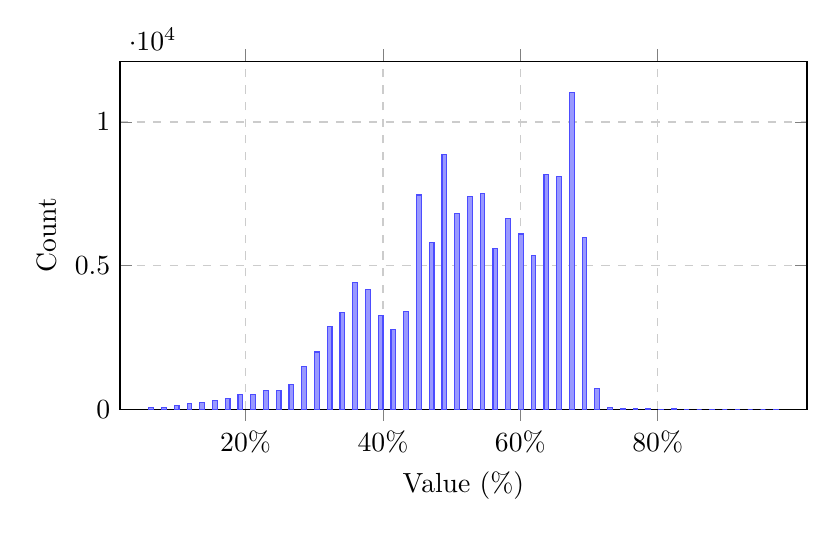
\begin{tikzpicture}
\begin{axis}[
  ybar,
  bar width=1.7073pt,
  xlabel={Value (\%)},
  ylabel={Count},
  xtick={20.0,40.0,60.0,80.0},
  xticklabel={$\pgfmathprintnumber[fixed,precision=1]{\tick}\%$},
  ymin=0,
  enlarge x limits=0.05,
  grid=major,
  grid style={dashed, gray!40},
  width=0.85\linewidth,
  height=6cm,
]
\addplot[fill=blue!40, draw=blue!70] coordinates {
  (6.2513, 53)
  (8.1071, 61)
  (9.9629, 128)
  (11.8187, 188)
  (13.6745, 245)
  (15.5303, 286)
  (17.3861, 356)
  (19.2419, 500)
  (21.0977, 515)
  (22.9535, 647)
  (24.8093, 649)
  (26.6651, 861)
  (28.5209, 1495)
  (30.3767, 1990)
  (32.2325, 2873)
  (34.0883, 3375)
  (35.9441, 4423)
  (37.7999, 4172)
  (39.6557, 3254)
  (41.5115, 2787)
  (43.3673, 3396)
  (45.2230, 7458)
  (47.0788, 5804)
  (48.9346, 8859)
  (50.7904, 6823)
  (52.6462, 7402)
  (54.5020, 7513)
  (56.3578, 5592)
  (58.2136, 6626)
  (60.0694, 6099)
  (61.9252, 5347)
  (63.7810, 8161)
  (65.6368, 8092)
  (67.4926, 11015)
  (69.3484, 5970)
  (71.2042, 728)
  (73.0600, 45)
  (74.9158, 19)
  (76.7716, 13)
  (78.6274, 3)
  (80.4832, 1)
  (82.3389, 3)
  (84.1947, 0)
  (86.0505, 0)
  (87.9063, 1)
  (89.7621, 0)
  (91.6179, 0)
  (93.4737, 0)
  (95.3295, 0)
  (97.1853, 1)
};
\end{axis}
\end{tikzpicture}
